\chapter{Conceptos preliminares}
\label{cap:conceptos}

Antes de entrar en la definición formal del problema, el estado del arte y el desarrollo del clasificador, conviene fijar algunos conceptos básicos. Este capítulo está pensado para que cualquier lector con formación en Informática, aunque no sea especialista en ciberseguridad, pueda seguir el resto de la memoria. Se explican primero las ideas generales (qué es la ciberseguridad en redes y cómo se detectan los ataques) y, a continuación, las piezas concretas que usa este trabajo: NetFlow, el dataset UGR'16, el aprendizaje automático clásico, los modelos de lenguaje y las métricas de evaluación.

\section{Ciberseguridad y tráfico de red}
\label{sec:concep_ciberseguridad}

La ciberseguridad se ocupa de proteger los sistemas informáticos y la información que manejan frente a usos no autorizados o maliciosos. En el contexto de las redes de comunicaciones, esto incluye vigilar el tráfico que circula entre máquinas para detectar actividad que no corresponde al funcionamiento normal de la organización.

La idea de analizar el tráfico de red para detectar comportamientos maliciosos parte de una observación sencilla: muchos ataques dejan rastro en la forma en que las máquinas se comunican. Aunque un atacante intente pasar desapercibido, sus acciones suelen generar conexiones que se desvían de lo habitual. Por ejemplo, un equipo que de repente contacta con cientos de máquinas distintas, o que envía una cantidad de conexiones muy superior a la normal hacia un mismo servicio, está mostrando un comportamiento que se puede observar y medir, incluso sin saber exactamente qué se está transmitiendo.

Los tipos de actividad maliciosa que pueden aparecer en una red son muy variados. Entre los más habituales están los \emph{escaneos}, en los que un origen explora qué máquinas o qué servicios están disponibles, los intentos de \emph{denegación de servicio}, que buscan saturar un servicio con un volumen de tráfico muy alto, los equipos \emph{comprometidos} que pasan a formar parte de una red controlada por un atacante, o las \emph{campañas automatizadas}, como el envío masivo de correo. No es necesario, por ahora, entrar en las familias concretas que contiene el dataset utilizado en este trabajo. Basta con quedarse con la idea de que cada tipo de ataque tiende a producir un patrón de tráfico característico, y que ese patrón es lo que se intenta reconocer.

El tráfico normal de una red real es enorme y muy diverso. Por eso, el reto no es solo reconocer un comportamiento sospechoso, sino distinguirlo del ruido de fondo legítimo, que puede parecerse mucho a un ataque en algunos casos. Esta dificultad es la que da sentido a los sistemas de detección que se describen a continuación.

\section{Sistemas de detección de intrusiones}
\label{sec:concep_ids}

Un sistema de detección de intrusiones (IDS, por sus siglas en inglés \emph{Intrusion Detection System}) es una herramienta cuyo objetivo es identificar actividad maliciosa o no autorizada dentro de un sistema o una red. Cuando el IDS analiza el tráfico que circula por la red se habla de un IDS de red (NIDS), que es el tipo de enfoque relevante para este trabajo.

De forma general, los IDS se dividen en dos grandes familias según cómo deciden qué es un ataque \cite{garciateodoro2009anomaly}:

\begin{itemize}
  \item \textbf{Detección basada en firmas.} Se dispone de una base de datos de patrones conocidos (firmas) que describen ataques ya identificados. El sistema compara el tráfico con esas firmas y, si encuentra una coincidencia, genera una alerta. Su principal ventaja es que es muy fiable con ataques conocidos y produce pocos falsos positivos. Su limitación es que no detecta ataques nuevos: si no existe una firma para una amenaza, esta pasa desapercibida.
  \item \textbf{Detección basada en anomalías.} En lugar de buscar firmas concretas, se construye un modelo de lo que se considera comportamiento normal y se marca como sospechoso todo lo que se desvía de ese modelo \cite{chandola2009anomaly}. Su ventaja es que puede detectar amenazas no vistas antes, ya que no depende de conocer el ataque de antemano. Su limitación es que suele generar más falsos positivos, porque no todo lo que se sale de lo normal es necesariamente un ataque.
\end{itemize}

El enfoque desarrollado en este TFG está más cerca de la detección basada en anomalías y, sobre todo, en el comportamiento del tráfico. No se utilizan firmas de ataques concretos ni se depende de conocer de antemano cada amenaza. En su lugar, se estudia cómo se comporta el tráfico (cuántos destinos contacta un origen, cómo se reparte la actividad, qué servicios se usan) y se definen reglas que describen esos comportamientos. La diferencia importante respecto a un detector de anomalías puramente estadístico es que aquí cada decisión va acompañada de una explicación: no solo se dice que algo es anómalo, sino qué señal concreta lo ha provocado.

Este tipo de detección suele requerir algo más que observar cada flujo de manera aislada. Un único registro puede corresponder a una comunicación legítima y no mostrar ninguna señal claramente maliciosa, mientras que el comportamiento sospechoso aparece al analizar varios flujos relacionados durante un mismo intervalo de tiempo. Por este motivo, es habitual agrupar el tráfico en ventanas temporales y estudiar características agregadas, como el número de conexiones, la cantidad de destinos o puertos contactados y la concentración del tráfico sobre un mismo objetivo.

A partir de esas relaciones pueden reconocerse patrones generales. En un \emph{escaneo vertical}, un mismo origen prueba numerosos puertos de un único destino, mientras que en un \emph{escaneo horizontal} contacta muchos destinos a través de un mismo servicio. Un ataque de denegación de servicio concentra una actividad especialmente intensa contra un objetivo, y una botnet puede manifestarse mediante varios equipos que actúan de forma parecida o coordinada. También resulta útil el concepto de \emph{fan-out}, que representa el número de destinos distintos contactados por un mismo origen. Estos comportamientos se presentan aquí únicamente de forma introductoria, ya que su interpretación mediante ventanas y contexto se desarrolla con mayor detalle en los capítulos posteriores.

La Figura~\ref{fig:ids_firmas_anomalias} compara de forma esquemática los dos enfoques, el basado en firmas y el basado en anomalías.

\begin{figure}[!htbp]
\centering
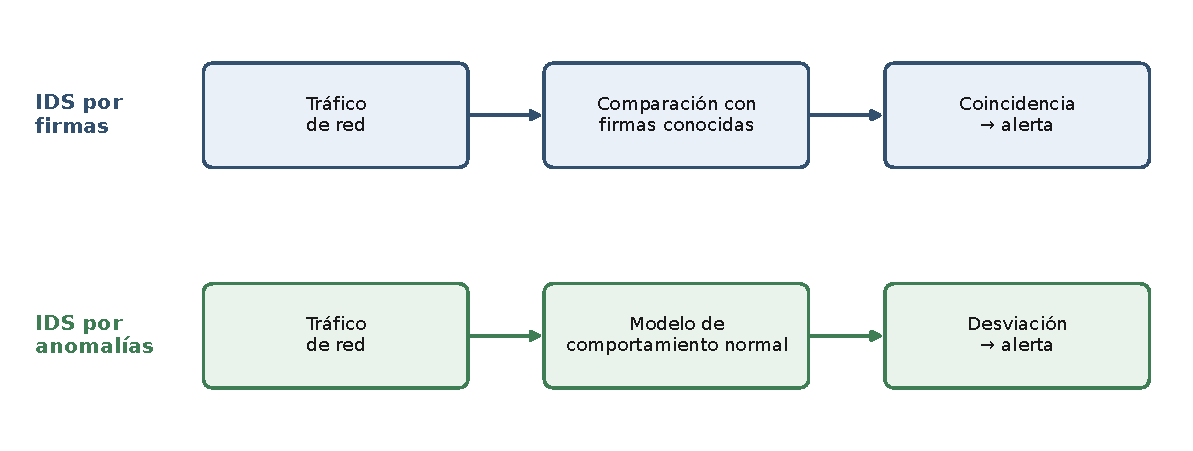
\includegraphics[width=0.9\textwidth]{imagenes/fig_ids_firmas_vs_anomalias.pdf}
\caption{Comparación esquemática entre un IDS basado en firmas y un IDS basado en anomalías. Fuente: elaboración propia.}
\label{fig:ids_firmas_anomalias}
\end{figure}

\section{Tráfico NetFlow}
\label{sec:concep_netflow}

NetFlow es una tecnología, originalmente desarrollada por Cisco, que resume la actividad de una red en forma de \emph{flujos} \cite{rfc3954}. Un flujo agrupa los paquetes que pertenecen a una misma comunicación (por ejemplo, los que comparten el mismo origen, destino, puertos y protocolo) y genera por cada uno un registro con sus metadatos. En lugar de guardar todo el contenido que circula por la red, NetFlow guarda un resumen por conexión.

La información que recoge un flujo NetFlow incluye, de forma general:

\begin{itemize}
  \item las direcciones \textbf{IP de origen y de destino}.
  \item los \textbf{puertos} de origen y de destino, que identifican el servicio utilizado (por ejemplo, el puerto 22 para SSH o el 25 para el correo).
  \item el \textbf{protocolo} de transporte (TCP, UDP, etc.).
  \item la \textbf{duración} del flujo.
  \item el número de \textbf{paquetes} y de \textbf{bytes} intercambiados.
  \item las \textbf{flags} TCP, cuando corresponde, que indican el tipo de los paquetes (por ejemplo, intentos de conexión).
\end{itemize}

La Figura~\ref{fig:flujo_netflow} muestra un esquema de flujo de NetFlow, y la Tabla~\ref{tab:campos_netflow} resume los campos principales que se utilizan en este trabajo. Además de los campos de metadatos, cada traza incluye una \textbf{etiqueta} que indica si corresponde a tráfico normal o a un tipo concreto de ataque. Esa etiqueta se usa solo para evaluar el rendimiento del detector, no para entrenarlo.

\begin{figure}[!htbp]
\centering
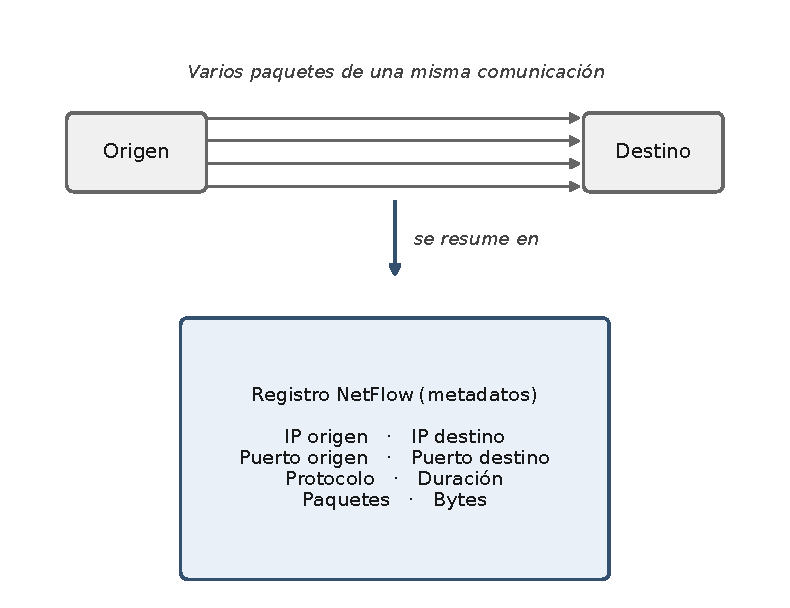
\includegraphics[width=0.65\textwidth]{imagenes/fig_flujo_netflow.pdf}
\caption{Esquema de un flujo NetFlow: varios paquetes de una comunicación se resumen en un registro de metadatos. Fuente: elaboración propia.}
\label{fig:flujo_netflow}
\end{figure}

\begin{table}[!htbp]
\centering
\small
\begin{tabular}{|l|p{8.5cm}|}
\hline
\textbf{Campo} & \textbf{Descripción} \\
\hline
Tiempo (\emph{timestamp}) & Marca temporal de inicio del flujo. \\
\hline
IP de origen & Dirección de la máquina que inicia la comunicación. \\
\hline
IP de destino & Dirección de la máquina contactada. \\
\hline
Puerto de origen & Puerto desde el que se emite la comunicación. \\
\hline
Puerto de destino & Puerto contactado, identifica el servicio (por ejemplo, 22 para SSH). \\
\hline
Protocolo & Protocolo de transporte (TCP, UDP, etc.). \\
\hline
Duración & Tiempo que dura el flujo. \\
\hline
Paquetes & Número de paquetes intercambiados en el flujo. \\
\hline
Bytes & Volumen de datos del flujo. \\
\hline
Banderas (\emph{flags}) & Banderas TCP, cuando corresponde, que indican el tipo de los paquetes. \\
\hline
Etiqueta (\emph{label}) & Clase real de la traza (normal o tipo de ataque). Se usa solo para evaluar. \\
\hline
\end{tabular}
\caption{Campos principales de una traza NetFlow utilizados en el análisis.}
\label{tab:campos_netflow}
\end{table}

El punto clave de NetFlow es lo que \emph{no} contiene: no guarda el contenido (\emph{payload}) de la comunicación. No se puede ver el texto de un correo, el cuerpo de una petición web ni los datos concretos que se transmiten. Solo se dispone de metadatos sobre quién habla con quién, cuándo, con qué servicio y con qué volumen.

Esta característica tiene dos caras. Por un lado, es muy útil: permite analizar redes muy grandes con un coste razonable y sin invadir la privacidad de los usuarios, ya que no se inspecciona el contenido. Por otro lado, es una limitación importante, porque hay ataques cuya naturaleza solo se aprecia mirando el contenido. Como se verá más adelante, esto hace que algunas familias de ataque sean más fáciles de caracterizar a partir de su comportamiento que otras. Trabajar con NetFlow obliga, por tanto, a apoyarse en \emph{cómo} se comunica una máquina, y no en \emph{qué} comunica.

\section{Dataset UGR'16}
\label{sec:concep_ugr16}

UGR'16 es un conjunto de datos público creado específicamente para facilitar la evaluación de sistemas de detección de intrusiones en red \cite{ugr16}. Su principal interés frente a otros conjuntos de datos más antiguos es que se construyó a partir de \textbf{tráfico real} recogido durante más de cuatro meses en la red de un proveedor español de servicios de Internet (ISP). La captura se realizó mediante varios colectores NetFlow v9 situados en distintos puntos de la infraestructura, obteniendo más de 16.900 millones de registros de flujo. Las direcciones IP fueron anonimizadas para proteger la privacidad de los usuarios, pero se mantuvieron las características necesarias para estudiar el comportamiento de las comunicaciones. Al proceder de una red en producción, el tráfico incluye variaciones de volumen, conexiones legítimas, protocolos distintos, actividad periódica y comportamientos poco frecuentes que difícilmente aparecerían en un entorno de laboratorio. Esta variedad introduce ruido y situaciones ambiguas, pero también permite evaluar un detector en unas condiciones más cercanas a las que encontraría en un escenario real.

El dataset está formado por registros NetFlow, donde cada fila representa de forma resumida una comunicación observada en la red. Entre los datos disponibles se encuentran la marca temporal, la duración del flujo, las direcciones y puertos de origen y destino, el protocolo, las banderas de la conexión y el número de paquetes y bytes intercambiados. Junto al tráfico de fondo, UGR'16 contiene \textbf{ataques y anomalías etiquetados} pertenecientes a distintas familias, entre ellas ataques de denegación de servicio, botnets y diferentes tipos de escaneo. Parte de estos ataques se generó de forma controlada sobre la propia infraestructura del ISP, de manera que quedaran mezclados con el tráfico real, mientras que otras anomalías fueron identificadas posteriormente durante el análisis del conjunto de datos.

Cada registro incorpora además una etiqueta que indica si el flujo pertenece al tráfico de fondo, denominado \emph{background}, o a una familia concreta de ataque. Estas etiquetas se utilizan como referencia para comparar posteriormente las predicciones del sistema con la clase asignada a cada traza. A partir de esta comparación se calculan los verdaderos positivos, falsos positivos, falsos negativos y verdaderos negativos, así como las métricas de precisión, recall y $F_1$.

Es importante diferenciar entre la información utilizada para detectar y la empleada para evaluar. La etiqueta no se proporciona al clasificador como una característica de entrada ni interviene en la decisión sobre si un flujo es normal o malicioso. El detector trabaja únicamente con los campos y patrones observables del tráfico, como los orígenes y destinos, los puertos, el protocolo, el volumen y el contexto temporal. Las etiquetas se consultan una vez ejecutado el sistema para comprobar sus resultados. Aun así, deben entenderse como la referencia proporcionada por UGR'16, ya que el tráfico marcado como \emph{background} puede contener comportamientos atípicos que no hubieran sido identificados o etiquetados originalmente.

Otra característica útil de UGR'16 es su organización temporal. Los datos se dividen en dos bloques principales y, dentro de ellos, en capturas semanales. El conjunto de calibración reúne tráfico de fondo real recogido entre marzo y junio de 2016, mientras que el conjunto de prueba contiene tráfico de julio y agosto, combinando actividad real con ataques introducidos de forma controlada. Esta duración permite estudiar variaciones que no se aprecian en capturas breves, como las diferencias entre el día y la noche, los días laborables y los fines de semana, o los cambios que se producen entre semanas. Para este trabajo resulta especialmente importante porque permite diseñar y evaluar el detector sobre una captura concreta y comprobar después si las reglas obtenidas se mantienen sobre periodos diferentes. El detalle de las capturas seleccionadas, su distribución y las semanas utilizadas se presenta más adelante, en el capítulo de herramientas y datos. Aquí basta con entender por qué UGR'16 constituye una base adecuada para el trabajo: contiene tráfico real y prolongado en el tiempo, ofrece información estructurada en forma de flujos, incorpora varias familias de ataque etiquetadas y permite plantear experimentos de generalización temporal.

\section{Aprendizaje automático clásico}
\label{sec:concep_ml}

El aprendizaje automático (\emph{Machine Learning}) agrupa un conjunto de técnicas que permiten que un programa aprenda a realizar una tarea a partir de ejemplos, en lugar de seguir reglas escritas a mano \cite{hastie2009elements}. En la modalidad \textbf{supervisada}, que es la relevante aquí, se parte de un conjunto de datos etiquetados (entradas con su respuesta correcta) y se entrena un modelo para que aprenda a predecir la etiqueta de ejemplos nuevos. Aplicado a la clasificación de tráfico de red, esto significa entrenar un modelo con flujos ya etiquetados como normales o como un tipo de ataque, de forma que después pueda clasificar flujos que no ha visto.

Existen muchos modelos clásicos de clasificación, y varios de ellos se usan habitualmente en detección de intrusiones \cite{buczak2016survey}. Entre los más conocidos están:

\begin{itemize}
  \item \textbf{K vecinos más cercanos (KNN):} clasifica cada ejemplo según las etiquetas de los ejemplos más parecidos a él.
  \item \textbf{Máquinas de vectores soporte (SVM):} buscan una frontera que separe lo mejor posible las distintas clases \cite{cortes1995support}.
  \item \textbf{Regresión logística:} estima la probabilidad de que un ejemplo pertenezca a una clase a partir de una combinación de sus características.
  \item \textbf{Redes neuronales / perceptrón multicapa (MLP):} modelos formados por capas de neuronas artificiales capaces de aprender relaciones no lineales entre las características.
\end{itemize}

Estos modelos pueden ofrecer muy buenos resultados, pero comparten una característica importante para este trabajo: necesitan datos etiquetados para entrenarse y, en muchos casos, su decisión es difícil de interpretar caso a caso. En este TFG el aprendizaje automático clásico \textbf{no} es el enfoque principal: se utiliza únicamente como \textbf{comparación experimental} (\emph{baseline}), es decir, como referencia frente a la que situar el rendimiento del clasificador basado en reglas. El detector propuesto, en cambio, no se entrena con etiquetas, sino que aplica reglas conductuales pensadas para ser explicables.

\section{Modelos de lenguaje y NotebookLM}
\label{sec:concep_llm}

Los modelos de lenguaje grandes (LLM, \emph{Large Language Models}) son modelos entrenados sobre grandes cantidades de texto que aprenden a predecir y generar lenguaje natural. La mayoría se basa en la arquitectura \emph{transformer} \cite{vaswani2017attention}, y los modelos más recientes han mostrado una notable capacidad para resumir información, responder preguntas y razonar sobre textos a partir de las instrucciones que reciben \cite{brown2020language}. A alto nivel, pueden entenderse como asistentes capaces de leer documentación, sintetizarla y ayudar a explorar un problema.

En este trabajo se utiliza \textbf{NotebookLM} \cite{notebooklm}, una herramienta basada en modelos de lenguaje que permite cargar documentos y hacer preguntas sobre ellos, de modo que las respuestas se apoyan en ese material. Funciona como un sistema de \textbf{generación aumentada por recuperación} (RAG, \emph{Retrieval-Augmented Generation}): en lugar de responder solo con lo que el modelo aprendió durante su entrenamiento, primero recupera los fragmentos relevantes de los documentos que se le han dado y, sobre esa base, genera la respuesta. Esto lo hace adecuado para trabajar sobre el material concreto del proyecto, ya que las respuestas se ciñen a las fuentes cargadas. Su papel en el TFG es servir de \textbf{apoyo al análisis}: ayuda a revisar documentación, resumir patrones observados, comparar ventanas de tráfico y formular hipótesis sobre qué señales caracterizan a cada ataque. Esas hipótesis se transforman después en reglas que se comprueban con código.

Un punto se mantiene durante toda la memoria: \textbf{NotebookLM y los LLM no detectan ataques ni sustituyen al clasificador}. No deciden qué tráfico es malicioso. La detección final la realiza siempre el clasificador contextual basado en reglas, que es un algoritmo explícito y revisable. Esta separación es deliberada: permite aprovechar la capacidad de los modelos de lenguaje para interpretar y documentar, sin que el sistema dependa de una respuesta generada por un modelo difícil de auditar.

\section{Métricas de evaluación}
\label{sec:concep_metricas}

Para valorar si un detector funciona bien no basta con mirar cuántas veces acierta en total. Hacen falta métricas que tengan en cuenta los distintos tipos de error \cite{sokolova2009systematic}. Al comparar la salida del sistema con la etiqueta real, cada traza cae en una de cuatro situaciones:

\begin{itemize}
  \item \textbf{Verdadero positivo (VP):} el sistema marca ataque y realmente era ataque.
  \item \textbf{Falso positivo (FP):} el sistema marca ataque, pero era tráfico normal (una falsa alarma).
  \item \textbf{Falso negativo (FN):} el sistema no detecta un ataque que sí existía (se le escapa).
  \item \textbf{Verdadero negativo (VN):} el sistema marca normal y realmente era normal.
\end{itemize}

A partir de estos valores se definen las métricas más usadas. La \textbf{precisión} mide qué parte de lo que el sistema marca como ataque es correcto, el \textbf{recall} (o exhaustividad) mide qué parte de los ataques reales llega a detectar, y la medida \textbf{F1} combina ambas en un único valor, como su media armónica:

\[
P = \frac{VP}{VP + FP}, \qquad
R = \frac{VP}{VP + FN}, \qquad
F_1 = \frac{2 \, P \, R}{P + R}.
\]

La Tabla~\ref{tab:metricas_prf1} resume estas tres métricas, con su fórmula y su interpretación en detección de intrusiones.

\begin{table}[!htbp]
\centering
\small
\begin{tabular}{|l|c|p{3.6cm}|p{4.6cm}|}
\hline
\textbf{Métrica} & \textbf{Fórmula} & \textbf{Qué mide} & \textbf{Interpretación en detección de intrusiones} \\
\hline
Precisión & $\frac{VP}{VP + FP}$ & Parte de lo marcado como ataque que es correcto. & Una precisión alta significa pocas falsas alarmas. \\
\hline
Recall & $\frac{VP}{VP + FN}$ & Parte de los ataques reales que llega a detectar. & Un recall alto significa que se escapan pocos ataques. \\
\hline
F1 & $\frac{2 \, P \, R}{P + R}$ & Media armónica de precisión y recall. & Resume en un solo valor el equilibrio entre falsas alarmas y ataques no detectados. \\
\hline
\end{tabular}
\caption{Precisión, recall y F1: interpretación de las métricas utilizadas.}
\label{tab:metricas_prf1}
\end{table}

Estas métricas miran cosas distintas y conviene leerlas juntas. Una precisión alta indica que el sistema genera pocas falsas alarmas. Un recall alto indica que se le escapan pocos ataques. A menudo hay una tensión entre ambas: ser muy estricto reduce los falsos positivos pero puede aumentar los falsos negativos, y al revés. La medida $F_1$ es útil porque resume ese equilibrio en un solo número.

Por último, queda explicar por qué no se usa como métrica principal la \textbf{exactitud} (\emph{accuracy}), es decir, la proporción de aciertos sobre el total. En detección de intrusiones los datos suelen estar muy \textbf{desbalanceados}: la inmensa mayoría del tráfico es normal y solo una pequeña parte son ataques. En ese escenario, un sistema que clasificara absolutamente todo como tráfico normal obtendría una exactitud altísima, simplemente porque casi todo es normal, y aun así no detectaría ni un solo ataque. Por eso, en este trabajo se da prioridad a precisión, recall y $F_1$, que reflejan mejor la capacidad real de detección sobre las clases minoritarias.
